\chapter{Reference elements}

%------------------------------------------------------------------------------
\section{The reference triangle}

The reference~triangle\index{reference triangle} (Figure \ref{fig:reference_triangle})
is defined by the following three vertices:
\begin{equation}
  \begin{split}
    v^0 &= (0,0), \\
    v^1 &= (1,0), \\
    v^2 &= (0,1).
  \end{split}
\end{equation}
Note that this corresponds to a counter-clockwise orientation of the vertices in the plane.

The edges of the reference triangle are ordered following the convention that edge $e^i$ should be
opposite to vertex $v^i$ for $i=0,1,2$, with the vertices of each edge ordered to give a
counter-clockwise orientation of the triangle in the plane:
\begin{equation}
  \begin{split}
    e^0 &: (v^1, v^2), \\
    e^1 &: (v^2, v^0), \\
    e^2 &: (v^0, v^1).
  \end{split}
\end{equation}

\begin{figure}[htbp]
  \begin{center}
    \psfrag{x0}{$x_0$}
    \psfrag{x1}{$x_1$}
    \psfrag{v0}{$v^0$}
    \psfrag{v1}{$v^1$}
    \psfrag{v2}{$v^2$}
    \psfrag{p0}{$v^0 = (0,0)$}
    \psfrag{p1}{$v^1 = (1,0)$}
    \psfrag{p2}{$v^2 = (0,1)$}
    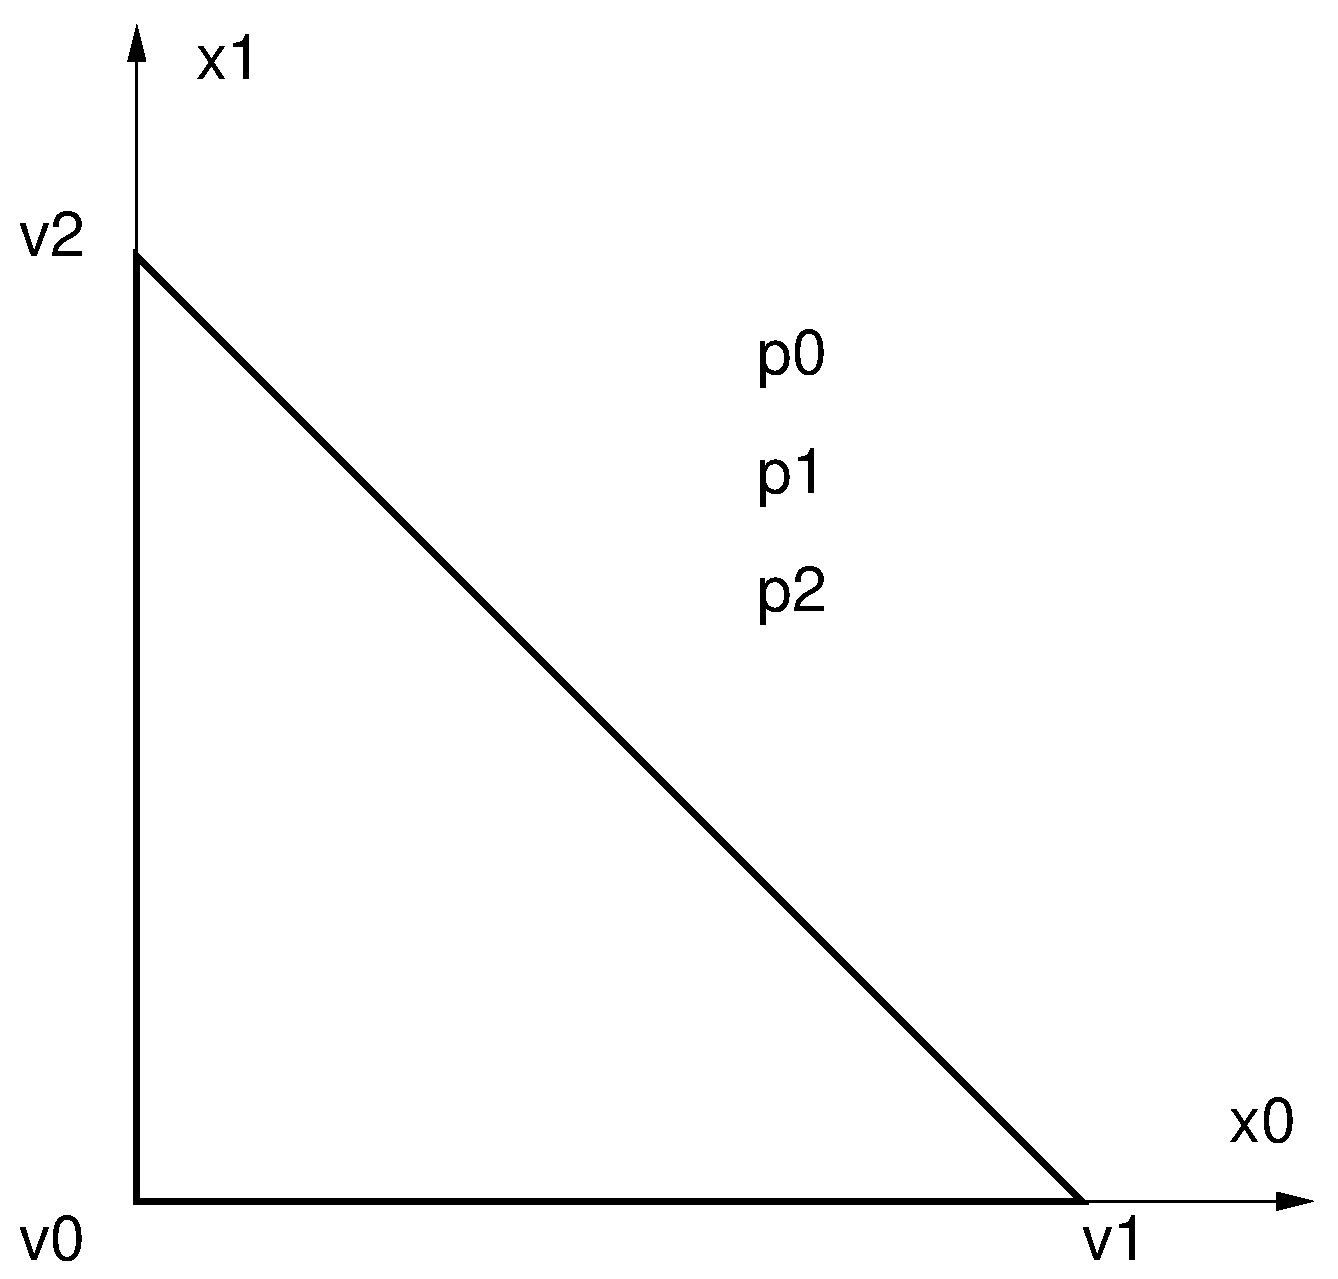
\includegraphics[width=8cm]{eps/reference_triangle.eps}
    \caption{Physical coordinates of the reference triangle.}
    \label{fig:reference_triangle}
  \end{center}
\end{figure}

\begin{figure}[htbp]
  \begin{center}
    \psfrag{v0}{$v^0$}
    \psfrag{v1}{$v^1$}
    \psfrag{v2}{$v^2$}
    \psfrag{e0}{$e^0$}
    \psfrag{e1}{$e^1$}
    \psfrag{e2}{$e^2$}
    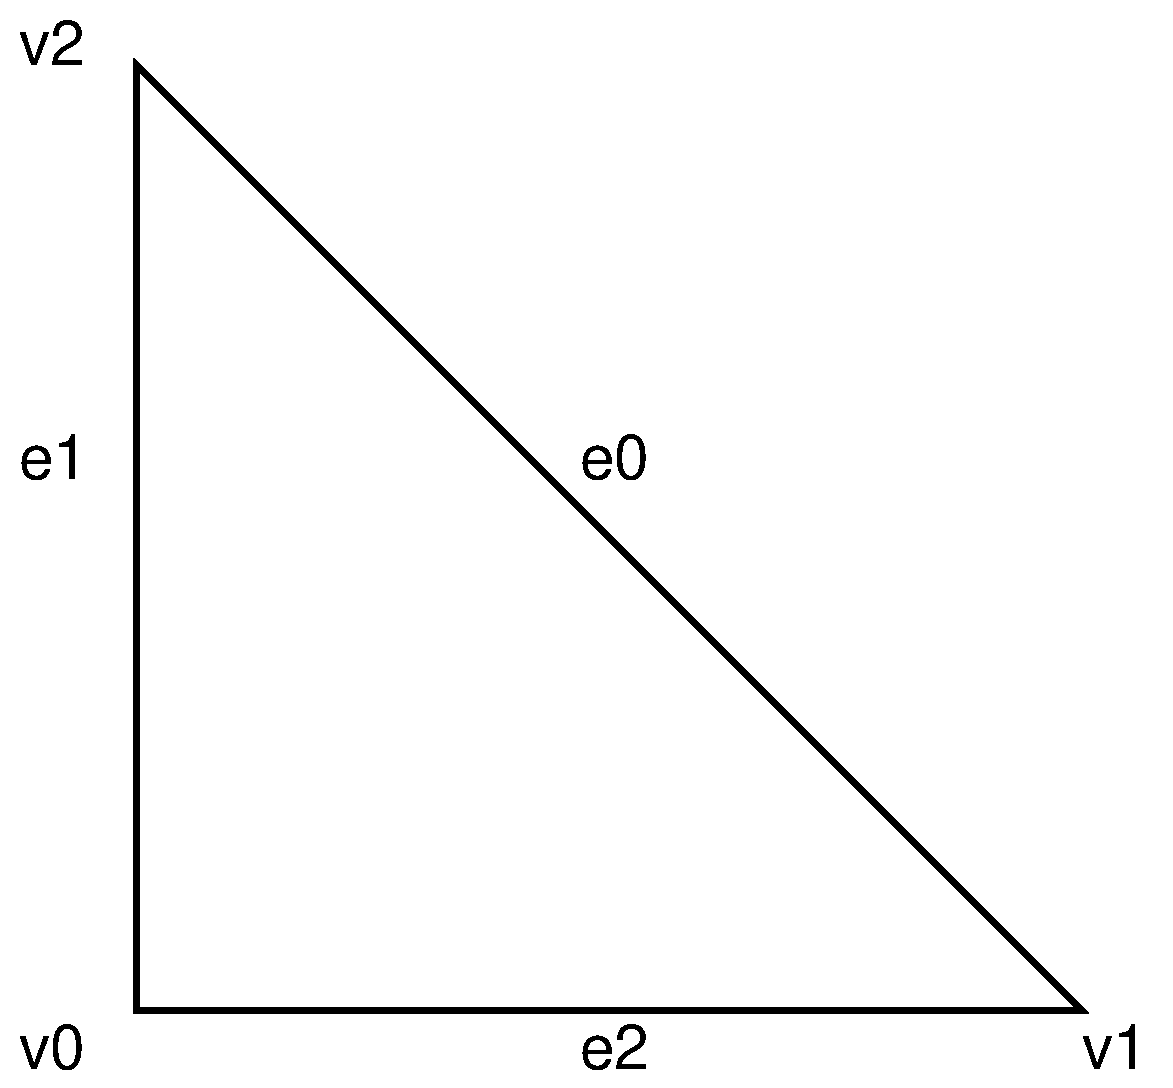
\includegraphics[width=8cm]{eps/reference_triangle_entities.eps}
    \caption{Ordering of mesh entities (vertices and edges) for the reference triangle.}
    \label{fig:reference_triangle_entities}
  \end{center}
\end{figure}

%------------------------------------------------------------------------------
\section{The reference tetrahedron}

The reference~tetrahedron\index{reference tetrahedron} (Figure \ref{fig:reference_tetrahedron})
is defined by the following four vertices:
\begin{equation}
  \begin{split}
    v^0 &= (0,0,0), \\
    v^1 &= (1,0,0), \\
    v^2 &= (0,1,0), \\
    v^4 &= (0,0,1).
  \end{split}
\end{equation}

The faces of the reference tetrahedron are ordered following the convention that face $f^i$ should be
opposite to vertex $v^i$ for $i=0,1,2,3$, with the vertices of each face ordered to give a
clockwise orientation of each face as seen from the outside of the tetrahedron and
the first vertex of face $f^i$ given by vertex $v^{i + 1 \mod 4}$:
\begin{equation}
  \begin{split}
    f^0 &: (v^1, v^3, v^2), \\
    f^1 &: (v^2, v^3, v^0), \\
    f^2 &: (v^3, v^1, v^0), \\
    f^3 &: (v^0, v^1, v^2).
  \end{split}
\end{equation}

The edges of the reference tetrahedron are ordered following the convention that edges $e^0, e^1, e^2$
should correspond to the edges of the reference triangle. Edges $e^3, e^4, e^5$ all ending up at vertex 
$v^3$ are ordered based on their first vertex:
\begin{equation}
  \begin{split}
    e^0 &: (v^1, v^2), \\
    e^1 &: (v^2, v^0), \\
    e^2 &: (v^0, v^1), \\
    e^3 &: (v^0, v^3), \\
    e^4 &: (v^1, v^3), \\
    e^5 &: (v^2, v^3).
  \end{split}
\end{equation}

The ordering of vertices on faces implicitly defines an ordering of edges
on faces by identifying an edge on a face with the opposite vertex on the face:
\begin{equation}
  \begin{split}
    f^0 &: (e^5, e^0, e^4), \\
    f^1 &: (e^3, e^1, e^5), \\
    f^2 &: (e^2, e^3, e^4), \\
    f^3 &: (e^0, e^1, e^2).
  \end{split}
\end{equation}
Note that the ordering of edges on $f^3$ is the same
as the ordering of edges on the reference triangle. Also note that the internal ordering
of vertices on edges does not always follow the orientation of the face (which is not possible).

\begin{figure}[htbp]
  \begin{center}
    \psfrag{x0}{$x_0$}
    \psfrag{x1}{$x_1$}
    \psfrag{x2}{$x_2$}
    \psfrag{v0}{$v^0$}
    \psfrag{v1}{$v^1$}
    \psfrag{v2}{$v^2$}
    \psfrag{v3}{$v^3$}
    \psfrag{p0}{$v^0 = (0,0,0)$}
    \psfrag{p1}{$v^1 = (1,0,0)$}
    \psfrag{p2}{$v^2 = (0,1,0)$}
    \psfrag{p3}{$v^3 = (0,0,1)$}
    \includegraphics[width=10cm]{eps/reference_tetrahedron.eps}
    \caption{Physical coordinates of the reference tetrahedron.}
    \label{fig:reference_tetrahedron}
  \end{center}
\end{figure}

\begin{figure}[htbp]
  \begin{center}
    \psfrag{v0}{$v^0$}
    \psfrag{v1}{$v^1$}
    \psfrag{v2}{$v^2$}
    \psfrag{v3}{$v^3$}
    \psfrag{e0}{$e^0$}
    \psfrag{e1}{$e^1$}
    \psfrag{e2}{$e^2$}
    \psfrag{e3}{$e^3$}
    \psfrag{e4}{$e^4$}
    \psfrag{e5}{$e^5$}
    \psfrag{f0}{$f^0$}
    \psfrag{f1}{$f^1$}
    \psfrag{f2}{$f^2$}
    \psfrag{f3}{$f^3$}
    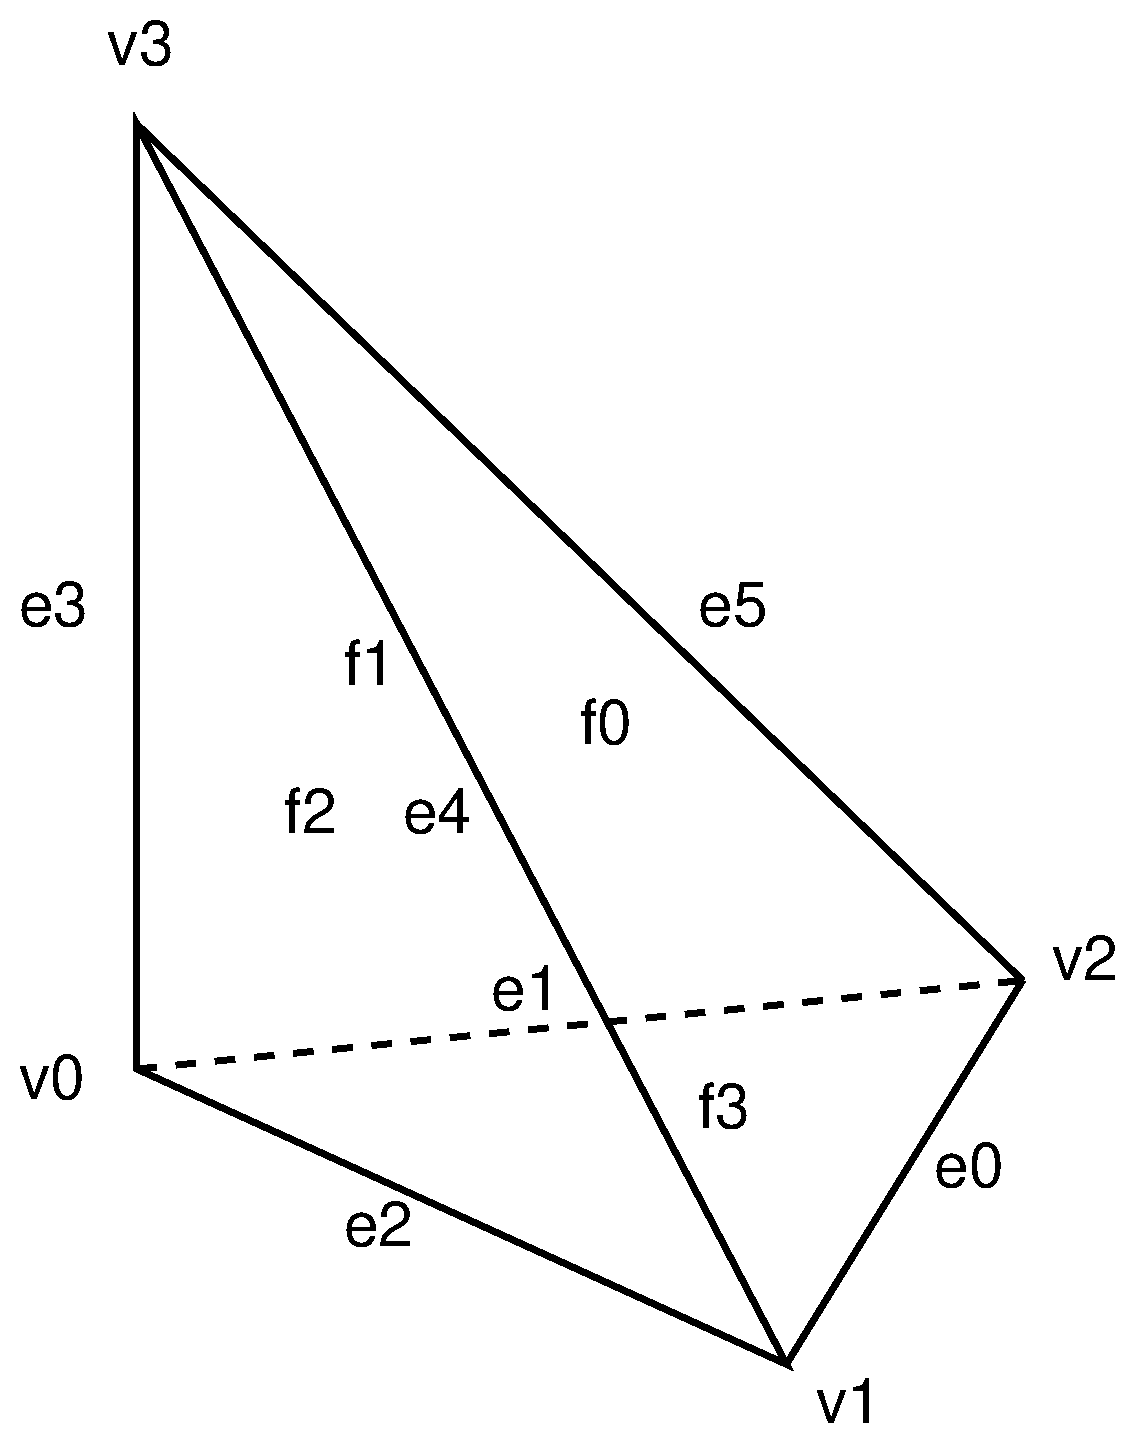
\includegraphics[width=10cm]{eps/reference_tetrahedron_entities.eps}
    \caption{Ordering of mesh entities (vertices, edges, faces) for the reference tetrahedron.}
    \label{fig:reference_tetrahedron_entities}
  \end{center}
\end{figure}

%------------------------------------------------------------------------------
\section{Ordering of degrees of freedom}

The local and global orderings of degrees of freedom or \emph{nodes} are
obtained by associating each node with a mesh entity, locally and
globally.

\subsection{Mesh entities}

We distinguish between mesh entities of different topological
dimensions:

\begin{center}
  \begin{tabular}{l|l}
    \emph{vertices} & topological dimension 0 \\
    \emph{edges}    & topological dimension 1 \\
    \emph{faces}    & topological dimension 2 \\
    \emph{cells}    & topological dimension 2 or 3
  \end{tabular}
\end{center}

A cell can be either a triangle or a tetrahedron depending on
the type of mesh. For a mesh consisting of triangles, the mesh
entities involved are vertices, edges and cells, and for a mesh
consisting of tetrahedrons, the mesh entities involved are vertices,
edges, faces and cells.

\subsection{Ordering among mesh entities}

With each mesh entity, there can be associated zero or more nodes and
the nodes are ordered locally and globally based on the topological
dimension of the mesh entity with which they are associated. Thus,
any nodes associated with vertices are ordered first and nodes
associated with cells last.

If more than one node is associated with a single mesh entity, the
internal ordering of the nodes associated with the mesh entity becomes
important, in particular for edges and faces, where the nodes of two
adjacent cells sharing a common edge or face must line up.

\subsection{Internal ordering on edges}

For edges containing more than one node, the nodes are ordered in the
direction from the first vertex ($v_e^0$) of the edge to the second
vertex ($v_e^1$) of the edge as in Figure \ref{fig:ordering,edges}.

\begin{figure}[htbp]
  \begin{center}
    \psfrag{v0}{$v_e^0$}
    \psfrag{v1}{$v_e^1$}
    \psfrag{n0}{$0$}
    \psfrag{n1}{$1$}
    \psfrag{n2}{$2$}
    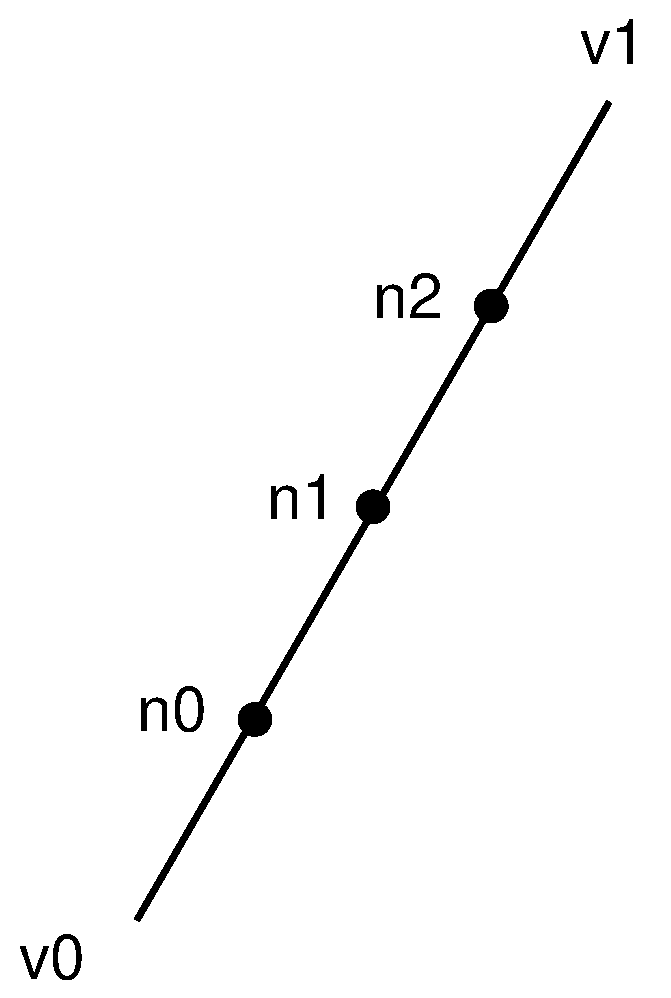
\includegraphics[width=5cm]{eps/edge_ordering.eps}
    \caption{Internal ordering of nodes on edges.}
    \label{fig:ordering,edges}
  \end{center}
\end{figure}

\subsection{Alignment of edges}

Depending on the orientation of any given cell, an edge on the cell
may be aligned or not aligned with the corresponding edge on the
reference cell if the vertices of the cell are mapped to the reference
cell. We define the \emph{alignment} of an edge with respect to a
cell to be $0$ if the edge is aligned with the orientation of the
reference cell and $1$ otherwise.

\textbf{Example 1:} The alignment of the first edge ($e^0$) on a
triangle is $0$ if the first vertex of the edge is the second vertex ($v^1$)
of the triangle.

\textbf{Example 2:} The alignment of the second edge ($e^1$) on a
tetrahedron is $0$ if the first vertex of the edge is the third vertex
($v^2$) of the tetrahedron.

If two cells share a common edge and the edge is aligned with one of
the cells and not the other, we must reverse the order in which the
local nodes are mapped to global nodes on one of the two cells. As a
convention, the order is kept if the alignment is $0$ and reversed if
the alignment is $1$.

\subsection{Internal ordering on faces}

For faces containing more than one node, the ordering of nodes is
nested going from the first to the third vertex and in each step going
from the first to the second vertex as in Figure \ref{fig:ordering,faces}.

\begin{figure}[htbp]
  \begin{center}
    \psfrag{v0}{$v_f^0$}
    \psfrag{v1}{$v_f^1$}
    \psfrag{v2}{$v_f^2$}
    \psfrag{n0}{$0$}
    \psfrag{n1}{$1$}
    \psfrag{n2}{$2$}
    \psfrag{n3}{$3$}
    \psfrag{n4}{$4$}
    \psfrag{n5}{$5$}
    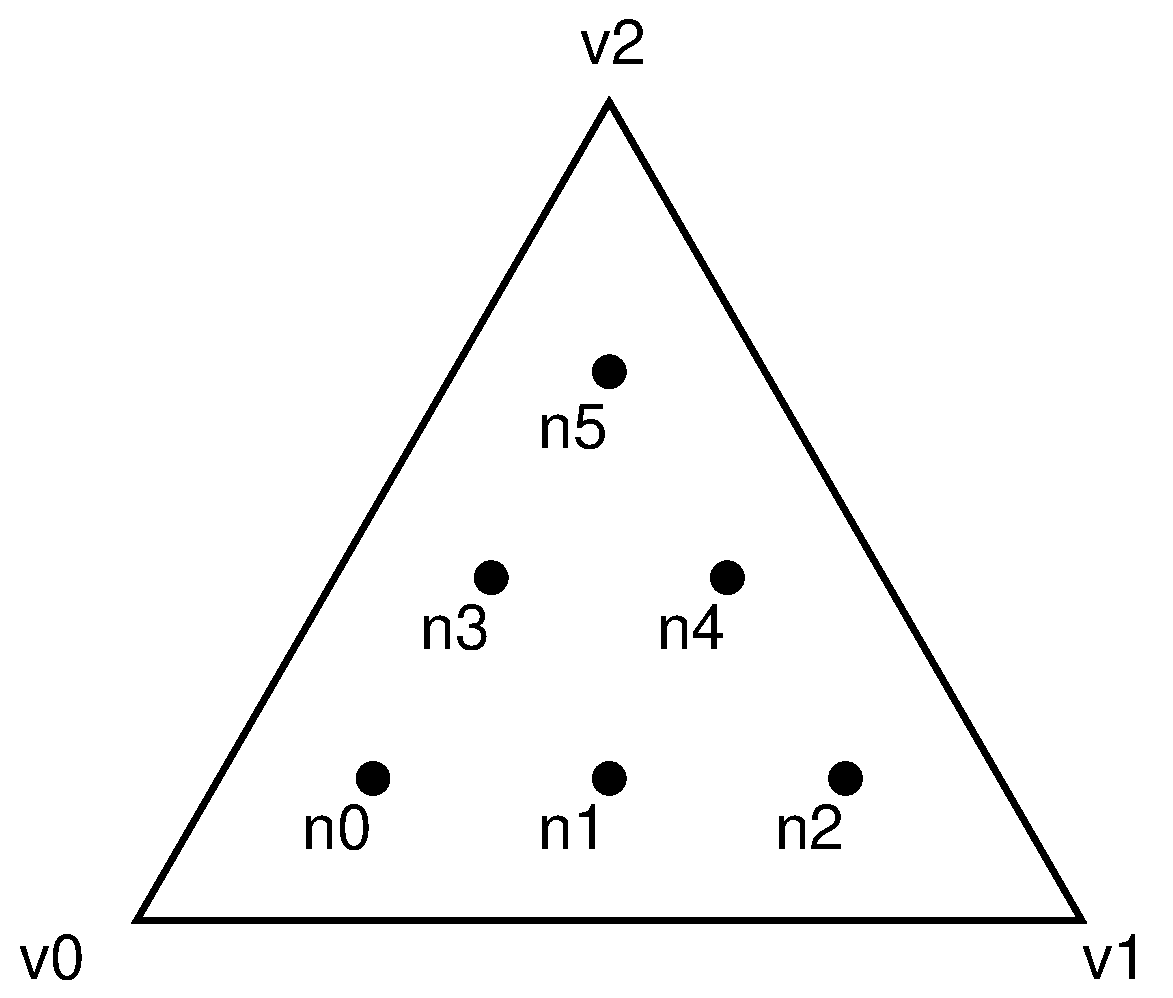
\includegraphics[width=10cm]{eps/face_ordering.eps}
    \caption{Internal ordering of nodes on faces.}
    \label{fig:ordering,faces}
  \end{center}
\end{figure}

\subsection{Alignment of faces}

There are six different ways for a face to be aligned on a
tetrahedron; there are three ways to pick the first edge of the face,
and once the first edge is picked, there are two ways to pick the
second edge. To define an alignment of faces as an integer between $0$
and $5$, we compare the ordering of edges on a face with the ordering
of edges on the corresponding face on the reference tetrahedron. If
the first edge of the face matches the first edge on the corresponding
face on the reference tetrahedron and also the second edge matches the
second edge on the reference tetrahedron, then the alignment is
$0$. If only the first edge matches, then the alignment is $1$. We
similarly define alignments~$2,3$ by matching the first and second
edges with the second and third edges on the corresponding face on the
reference tetrahedron, and alignments~$4,5$ by matching the first and
second edges with the third and first edges on the corresponding face
on the reference tetrahedron.

\textbf{Example 1:} The alignment of the first face of a tetrahedron
is $0$ if the first edge of the face is edge number~$5$ and the second
edge is edge number~$0$.

\textbf{Example 2:} The alignment of the first face of a tetrahedron
is $1$ if the first edge of the face is edge number~$5$ and the second
edge is not edge number~$0$. (It must then be edge number~$4$.)

\textbf{Example 3:} The alignment of the first face of a tetrahedron
is $4$ if the first edge of the face is edge number~$4$ and the second
edge is edge number~$5$.

\textbf{Example 4:} The alignment of the first face of a tetrahedron
is $5$ if the first edge of the face is edge number~$4$ and the second
edge is not edge number~$5$. (It must then be edge number~$0$.)
